%!TEX TS-program = xelatex
%!TEX encoding = UTF-8 Unicode
\documentclass[a4paper]{report}
%\usepackage[date=short,backend=biber]{apa}
\usepackage[hidelinks]{hyperref}
\usepackage{cite}
\usepackage[dutch]{babel}
\usepackage[a4paper, left=.8in, right=.8in, top=.8in, bottom=.6in]{geometry}
\usepackage[utf8]{inputenc}
\usepackage{fancyhdr}
\usepackage{titlesec}
\usepackage{geometry}
\usepackage{graphicx}
\usepackage{etoolbox}
\usepackage{listings}
\usepackage[x11names]{xcolor}
\usepackage{nameref}
\usepackage{tcolorbox}
\usepackage{textcomp}
\usepackage{helvet}
\usepackage{colortbl}
\usepackage{enumitem}
\usepackage{tabularx}
\usepackage{pgf-pie}  
\usepackage{float}
\usepackage{pdfpages}
\usepackage{pgfplots}
\usepackage{multicol}

% Variables
\newcommand{\latestVersion}{2}


% Hyphenations
\hyphenation{soort-gelijk soort-gelijke}

% Double-page bibliography
\makeatletter
\renewenvironment{thebibliography}[1]
     {\renewcommand{\chapter}[2]{} % Removes the 'Chapter' heading
     \renewcommand{\addcontentsline}[3]{}
      \begin{multicols}{2}[]%
      \@mkboth{\MakeUppercase\refname}{\MakeUppercase\refname}%
      \list{\@biblabel{\@arabic\c@enumiv}}%
           {\settowidth\labelwidth{\@biblabel{#1}}%
            \leftmargin\labelwidth
            \advance\leftmargin\labelsep
            \@openbib@code
            \usecounter{enumiv}%
            \let\p@enumiv\@empty
            \renewcommand\theenumiv{\@arabic\c@enumiv}}%
      \sloppy
      \clubpenalty4000
      \@clubpenalty \clubpenalty
      \widowpenalty4000%
      \sfcode`\.\@m}
     {\def\@noitemerr
       {\@latex@warning{Empty `thebibliography' environment}}%
      \endlist\end{multicols}}
\makeatother
% Styling
\pagestyle{fancy}
\patchcmd{\chapter}{\thispagestyle{plain}}{\thispagestyle{fancy}}{}{}

\newcommand{\styledhref}[2]{%
    \href{#1}{\textcolor{blue}{\underline{#2}}} % blue and underlined
}

\fancyhf{}
\fancyhead[L]{ Team Zeilvis Helden }
\fancyhead[R]{Logboek }
\fancyfoot[R]{\thepage}

\titleformat{\chapter}[hang]
{\normalfont\huge\bfseries}{\thechapter.}{10pt}{\huge}
\titlespacing{\chapter}{0pt}{-30pt}{20pt}

\setlength{\parindent}{0.2em}

\textwidth=400pt
\geometry{
    left=25mm
}

\renewcommand{\contentsname}{Inhoudsopgave}

\newcommand{\learningstorycolor}{PaleGreen1}
\newcommand{\enablerstorycolor}{SkyBlue1}
\newcommand{\researchstorycolor}{LightSlateGray1}
\newcommand{\userstorycolor}{PeachPuff1}


\definecolor{codegreen}{rgb}{0,0.6,0}
\definecolor{codegray}{rgb}{0.5,0.5,0.5}
\definecolor{codepurple}{rgb}{0.58,0,0.82}
\definecolor{backcolour}{rgb}{0.95,0.95,0.92}

\lstdefinestyle{mystyle}{
    backgroundcolor=\color{backcolour},   
    commentstyle=\color{codegreen},
    keywordstyle=\color{magenta},
    numberstyle=\tiny\color{codegray},
    stringstyle=\color{codepurple},
    basicstyle=\ttfamily\footnotesize,
    breakatwhitespace=false,         
    breaklines=true,                 
    captionpos=b,                    
    keepspaces=true,                 
    numbers=left,                    
    numbersep=5pt,                  
    showspaces=false,                
    showstringspaces=false,
    showtabs=false,                  
    tabsize=2
}

\lstset{style=mystyle}

% Commands
\newcommand{\teambox}{
  \begin{tcolorbox}[hbox, colback=blue!5!white,colframe=blue!75!black,
    left=.1mm, right=.1mm, top=.1mm, bottom=.1mm, fontupper=\scriptsize\sffamily]
    Team Keuze
  \end{tcolorbox}
}

\newcommand{\personalbox}{
  \begin{tcolorbox}[hbox, colback=green!5!white,colframe=green!75!black,
    left=.1mm, right=.1mm, top=.1mm, bottom=.1mm, fontupper=\scriptsize\sffamily]
    Persoonlijke Keuze
  \end{tcolorbox}
}
\newcommand{\teamchoice}[1]{
  \section[ #1 ]{#1~\mbox{\raisebox{-2.5pt}{\teambox}}}
}

\newcommand{\personalchoice}[1]{
  \section[ #1 ]{#1~\mbox{\raisebox{-2.5pt}{\personalbox}}}
}

\newcommand{\timestamp}[1]{
  \mbox{\scriptsize \textbf{Datum:} #1} \smallbreak
}

% Document
\begin{document}


% Title Page
\begin{titlepage}
  \begin{center}
      \vspace*{.6cm}
      \Huge
      \textbf{ Gilde Logboek }\\
      \vspace{0.2cm}
      \small Vincent van Setten \\
      \small Zeilvis Helden (Team FairPhone)

      \normalsize


      \vspace{1cm}
      
\includegraphics[width=0.7\textwidth]{Images/zeilvis_helden.png}
      \vspace{1cm}
      \Large\\
      \textbf{In opdracht van}\\
      \large
      \textbf{Hogeschool Utrecht} \\
      
\includegraphics[width=0.2\textwidth]{Images/logouni.png}


      \vfill
    \end{center}
      \textbf{Student:} Vincent van Setten - 1734729 \\
      \textbf{Gilde:} TI Gilde, Groep D\\
      \textbf{Innovation Team:} Project FairPhone (499) \\
      \textbf{Document Versie(Iteratie):} \latestVersion \\
      \textbf{Datum:} \today \\
      \vspace{2cm}
\end{titlepage}



% ToC
\tableofcontents

\chapter{Versiebeheer}
\begin{table}[h]
    \centering
    \begin{tabular}{|c|c|c|p{5cm}|}
        \hline
        \textbf{Versie} & \textbf{Datum} & \textbf{Veranderingen}  \\
        \hline
        2.0   & 2023-12-13 & Iteratie 6 toegevoegd \\
        \hline
        1.0   & 2023-11-29 & Eerste Versie \\
        \hline

    \end{tabular}
    \caption{Versiebeheer}
\end{table}


\chapter{Introductie}
Dit document dient as logboek voor de taken gedaan in het Innovation project door Vincent van Setten.
Met dit logboek hoop ik inzicht te geven aan het werk dat ik heb gedaan in de verschillende sprints tijdens dit project.


\vspace{1.5cm}


% \chapter{Iteratie 0 (Template)}
% \begin{table}[H]
% \begin{tabularx}{0.5\textwidth}{|X|X|}
%   \hline
%   \cellcolor[HTML]{99ccff} \textbf{Periode:} & x \\ 
%   \hline
%   \cellcolor[HTML]{99ccff} \textbf{Aantal taken:} & x \\ 
%   \hline
%   \cellcolor[HTML]{99ccff} \textbf{Totaal uren:} & x \\ 
%   \hline
% \end{tabularx}
% \caption{Informatie Tabel}
% \label{table:it1:general}
% \end{table}


% Taak Example
% \begin{tcolorbox}[colback=white, colframe=darkgray, title=Example | (Type)]
% \begin{table}[H]
%     \centering
%   \begin{tabularx}{1\textwidth}{|X|X|}
%     \hline
%     \cellcolor[HTML]{ffcc99} \textbf{Taak} & \cellcolor[HTML]{ffcc99} \textbf{Acceptatie Criteria} \\ 
%     \hline
%     Lorem & Ipsum \\
%     \hline
    
%   \end{tabularx}
%   \caption{Example table}
% \label{table:1}
% \end{table}
% \end{tcolorbox}


\chapter{Sprint 1}
\section{Algemene Informatie}
\begin{table}[H]
\begin{tabularx}{0.6\textwidth}{|X|X|}
  \hline
  \cellcolor[HTML]{99ccff} \textbf{Periode:} & 2023-09-11 t/m 2023-09-22 \\ 
  \hline
  \cellcolor[HTML]{99ccff} \textbf{Aantal taken:} & 7 \\ 
  \hline
  \cellcolor[HTML]{99ccff} \textbf{Totaal uren:} & 48 \\ 
  \hline
\end{tabularx}
\caption{Informatie Tabel}
\label{table:it1:general}
\end{table}

Het doel van de eerste sprint was het inlezen over het project en de dingen die het afgelopen team heeft afgerond.
Dit hebben we gedaan door alle documentatie die beschikbaar was door te lezen en ons begrip te toetsen door de README in de 'Getting Started' repository te updaten, zodat deze duidelijker en gebruiksvriendelijker is voor een potentieel volgend team.

\section{User Stories \& Taken}
\begin{tcolorbox}[colback=white, coltitle=black, colframe=\learningstorycolor, title=\textbf{Learning Story: }Als developer wil ik de belangrijke aspecten van de context van het project begrijpen\, namelijk de terminologie\, code- en git-structuur\, en project omvang\, zodat ik snel en efficient kan beginnen met werken.]
  \begin{table}[H]
      \centering
    \begin{tabularx}{1\textwidth}{|X|X|}
      \hline
      \cellcolor[HTML]{ffcc99} \textbf{Taak} & \cellcolor[HTML]{ffcc99} \textbf{Acceptatie Criteria} \\ 
      \hline
      De GitHub organisatie doorspitten & Er is door de GitHub organisaties gekeken en er is een basaal begrip van wat elke repositories doen. \\
      \hline
      Verantwoordingsdocumenten vorige team doorgelezen & De verantwoordingsdocumenten van het vorige team zijn doorgelezen en er is een begrip over de keuzes die destijds door het team gemaakt zijn. \\
      \hline
      Sailfish OS Porter\'s Guide doorlezen & De porter's guide is doorgelezen en er is een basaal begrip van de context van het project. \\
      \hline
      Getting Started - Introductie updaten/herschrijven om het duidelijker te maken & De introductie van de getting started is aangepast en duidelijker voor het team.\\
      \hline
      Setup scripts doorlezen & Er is door de setup scripts gekeken en het is duidelijker wat de algemene stappen zijn in de build environment.\\
      \hline
    \end{tabularx}
    \caption{Learning Story: Project Context}
  \label{table:it1:story_learn}
  \end{table}
  \end{tcolorbox}

\begin{tcolorbox}[colback=white, coltitle=black, colframe=\enablerstorycolor, title=\textbf{Enabler Story: }Als developer wil ik een werkende build server\, zodat er gemakkelijk en snel SailfishOS builds gemaakt kunnen worden.]
  Tijdens het uitvoeren van deze taken gingen er allerlei dingen fout. De setup scripts, die gelijk zouden moeten werken, kregen errors. 
  Bij het handmatig bouwen van deze scripts volgens de stappen die beschreven stuitte we ook op errors.
  \begin{table}[H]
      \centering
    \begin{tabularx}{1\textwidth}{|X|X|}
      \hline
      \cellcolor[HTML]{ffcc99} \textbf{Taak} & \cellcolor[HTML]{ffcc99} \textbf{Acceptatie Criteria} \\ 
      \hline
      Setup scripts runnen & De setup scripts zijn uitgevoerd.\\
      \hline
      Manual Setup uitvoeren & De stappen in het 'manual installation' hoofdstuk zijn uitgevoerd.\\
      \hline
      
    \end{tabularx}
    \caption{Enabler Story: Build Server}
  \label{table:it1:story_buildserver}
  \end{table}
  \end{tcolorbox}

\chapter{Sprint 2}
\section{Algemene Informatie}
\begin{table}[H]
  \begin{tabularx}{0.6\textwidth}{|X|X|}
    \hline
    \cellcolor[HTML]{99ccff} \textbf{Periode:} & 2023-09-25 t/m 2023-10-06 \\ 
    \hline
    \cellcolor[HTML]{99ccff} \textbf{Aantal taken:} & 14 \\ 
    \hline
    \cellcolor[HTML]{99ccff} \textbf{Totaal uren:} & 48 \\ 
    \hline
  \end{tabularx}
  \caption{Informatie Tabel}
  \label{table:it2:general}
  \end{table}

In deze sprint hadden we de basis kennis van het project in onze zak en wisten we waar we aan moesten werken.
Ten eerste wilden we de errors oplossen en de build server goed werkend krijgen. Daarnaast wilden we graag de overdraagbaarheid verbeteren.
Hoewel het vorige team veel had gedocumenteerd, ging dit er van uit dat je bepaalde dingen al wist. Daarnaast klopten veel dingen in de stappen niet.
Dit wilden we graag verbeteren door de documentatie aan te passen.


\section{User Stories \& Taken}
\begin{tcolorbox}[colback=white, coltitle=black,colframe=\enablerstorycolor, title=\textbf{Enabler Story: }Als developer wil ik een werkende build server\, zodat er gemakkelijk en snel sailfishOS builds gemaakt kunnen worden.]
  \par\smallskip 
  Deze sprint heb ik voor deze user story de handmatige installatie meerdere keren uitgevoerd en alle errors ge-debugged. 
  Deze errors heb ik genoteerd en hiervoor de oplossingen beschreven. Dit heb ik uiteindelijk in de user guide gezet(zie bijlage \ref{bijlage:userguide}).
  Er was hierna nog een bug. De OS image werkte perfect, maar de boot image zorgde voor een bootloop. Deze wilde ik oplossen in Sprint 3.

  \begin{table}[H]
      \centering
    \begin{tabularx}{1\textwidth}{|X|X|}
      \hline
      \cellcolor[HTML]{ffcc99} \textbf{Taak} & \cellcolor[HTML]{ffcc99} \textbf{Acceptatie Criteria} \\ 
      \hline
      Werkende SailfishOS Image produceren & 
      \begin{enumerate}[leftmargin=.4cm, topsep=0cm, itemsep=.2cm]
        \item Er is een image gebouwd.
        \item De telefoon start op met de image.
        \item De telefoon werkt naar behoren met de image.
      \end{enumerate}
      \\
      \hline
      Droid-hal-version error oplossen  & De image kan gebouwd worden, zonder dat deze error zich opnieuw voordoet. \\
      \hline
      Kleine build errors oplossen in handmatige build stappen & De image kan handmatig gebouwd worden. \\
      \hline 
      Document opstellen met errors en daarbij de oplossing & Er is een document opgesteld met daarin alle errors die mogelijk voorkomen bij het handmatig bouwen van een image. \\  
      \hline
      User Guide aanvullen(met stappen van opzet buildserver) & Het user guide document is aangevuld met de stappen van hoe een build server opgezet moet worden vanaf het begin. \\ 
      \hline       
    \end{tabularx}
    \caption{Enabler Story: Build Server}
  \label{table:it2:story_buildserver}
  \end{table}
  \end{tcolorbox}
  \begin{tcolorbox}[colback=white, coltitle=black, colframe=\userstorycolor, title=\textbf{User Story: }Als developer wil ik een build omgeving hebben in een container\, zodat ik makkelijker kan ontwikkelen en makkelijker het project kan overdragen.]
    \par\smallskip 
    We wilden ook graag het opzetten van de buildserver in een Dockerfile stoppen, zodat potentiële volgende teams minder problemen zouden ondervinden tijdens dit proces.
    Na het oplossen van wat kleine problemen, zoals permissions, stuitte ik op het probleem dat bij een bepaalde stap de hele docker image vastliep.
    Deze stap was het 'updaten van de sources' van de package manager 'zypper. Dit gaf verder geen errors, ook niet tijdens het runnen met verbose output.
    Bij het initialiseren stopte hij gewoon.
    Tijdens de volgende sprint besloten we deze story over te dragen aan Rinske, omdat zij graag een technische taak wilde en ik deze taak niet heel leuk vond om te doen.
      \begin{table}[H]
        \centering
      \begin{tabularx}{1\textwidth}{|X|X|}
        \hline
        \cellcolor[HTML]{ffcc99} \textbf{Taak} & \cellcolor[HTML]{ffcc99} \textbf{Acceptatie Criteria} \\ 
        \hline
        Uitzoeken hoe een Dockerfile gestructureerd is & Er is onderzoek gedaan naar Dockerfiles en er is een begrip van hoe een Dockerfile werkt. \\
        \hline
        Handmatige stappen implementeren in bash bestand & Er is een bash bestand met hierin de stappen van het opzetten van de build omgeving. \\ 
        \hline 
        Docker testen & De Dockerfile en het bash bestand zijn getest. \\ 
        \hline 
        Docker permission problemen debuggen & Bij het runnen van de docker image zijn er geen problemen meer met permissions \\
        \hline 
        Zypper ref error onderzoeken & Onderzoeken waar het zypper ref probleem vandaan komt. \\ 
        \hline 
      \end{tabularx}
      \caption{User Story: Docker}
    \label{table:it2:story_docker}
    \end{table}
    \end{tcolorbox}
  \begin{tcolorbox}[colback=white, coltitle=black, colframe=\userstorycolor, title=\textbf{User Story: }Als gebruiker wil ik graag met de Fairphone mobiele data kunnen gebruiken\, zodat ik ook onderweg internet kan gebruiken.]
    \par\smallskip 
    Volgens het vorige team was het enige dat nog nodig was voor werkende 4G, het updaten van het besturingssysteem van 4.5.0.19 naar 4.5.0.24.
    Hier had Franky voornamelijk onderzoek naar gedaan. Aangezien ik toch nog bezig was met het debuggen van het build-process en constant nieuwe images aan het bouwen was, zou ik zijn stappen meenemen en kijken of dit werkte.
    Helaas werkte het net niet. Na een korte research stap vond ik dat er nog 2 kleine stappen miste. Na het toevoegen hiervan hadden we succesvol SailfishOS geüpdatet.
    Helaas loste dit niet de 4G problemen op.

    \begin{table}[H]
        \centering
      \begin{tabularx}{1\textwidth}{|X|X|}
        \hline
        \cellcolor[HTML]{ffcc99} \textbf{Taak} & \cellcolor[HTML]{ffcc99} \textbf{Acceptatie Criteria} \\ 
        \hline
        Update stappen, gevonden door Franky, testen &
          \begin{enumerate}[leftmargin=.4cm, topsep=0cm, itemsep=.2cm]
          \item Er is een SailfishOS image gebouwd met daarmee de stappen van Franky's oplossing geïmplementeerd.  
          \item Er is gekeken bij systeem informatie of er na de installatie een nieuwe versie van SailfishOS is geïnstalleerd.
          \end{enumerate} \\
        \hline
        Onderzoeken wat er nog mist in de stappen van Franky & Er zijn concrete stappen gevonden die nog nodig zijn om SailfishOS succesvol te kunnen updaten. \\
        \hline 
        Nieuwe image maken met gevonden oplossingen & Er is een nieuwe image gebouwd maar hierbij de nieuw-gevonden stappen. \\ 
        \hline 
        Testen of nieuwe image geüpdatet is & Er is gekeken bij systeem informatie of er na de installatie een nieuwe versie van SailfishOS is geïnstalleerd. \\
        \hline 
        
      \end{tabularx}
      \caption{User Story: Mobiele Data}
    \label{table:it2:story_mobiledata}
    \end{table}
    \end{tcolorbox}

\chapter{Sprint 3}
\section{Algemene Informatie}
\begin{table}[H]
  \begin{tabularx}{0.6\textwidth}{|X|X|}
    \hline
    \cellcolor[HTML]{99ccff} \textbf{Periode:} & 2023-10-09 t/m 2023-10-27 \\ 
    \hline
    \cellcolor[HTML]{99ccff} \textbf{Aantal taken:} & 6 \\ 
    \hline
    \cellcolor[HTML]{99ccff} \textbf{Totaal uren:} & 48 \\ 
    \hline
  \end{tabularx}
  \caption{Informatie Tabel}
  \label{table:it3:general}
  \end{table}

  Het doel van sprint 3 voor mij was vooral het laatste grote probleem oplossen in de buildserver.
  Hoewel we al een werkende OS image konden bouwen, werkte onze eigen gebouwde boot image not niet.
  Dit betekende dat we steeds met een oude boot image moesten flashen, wat betekent dat we daar geen aanpassingen in konden maken als dat nodig was.
   

\section{User Stories \& Taken}
\begin{tcolorbox}[colback=white, coltitle=black, colframe=\enablerstorycolor, title=\textbf{Enabler Story: }Als developer wil ik een werkende build server\, zodat er gemakkelijk en snel SailfishOS builds gemaakt kunnen worden.]
  Ik had een aantal ideeën over waarom de boot image wel of niet werkte. Ten eerste dacht ik dat de image mogelijk niet overschreven werd.
  Uiteindelijk bleek dat dit wel gebeurde. Toen ik uiteindelijk de details van de image bekeek met abootimg, zag ik dat de ram disk 0 bytes was.
  Tijdens het onderzoeken van de reden hiervoor, merkte ik ineens dat de output van make tijdens het maken van de kernel was errors gaf.
  Gek genoeg waren deze niet fatal en deze werden na een paar seconden weer van de console gecleared. 
  Deze errors gaven aan dat de programma's ccache en cpio niet gevonden werden. Deze stonden niet in de requirements gedocumenteerd.
  Na het installeren van deze packages, merkte ik dat de errors verdwenen waren. De boot image die hier uit kwam, had wel een ram disk.
  Het flashen hiervan werkte.

  \begin{table}[H]
      \centering
    \begin{tabularx}{1\textwidth}{|X|X|}
      \hline
      \cellcolor[HTML]{ffcc99} \textbf{Taak} & \cellcolor[HTML]{ffcc99} \textbf{Acceptatie Criteria} \\ 
      \hline
      Testen of aanpassingen in de installer van de boot image te zien zijn & Er is geconstateerd of de veranderingen die in de boot image source code zijn aangepast ook te zien zijn. \\ 
      \hline 
      Flashen via een sd kaart ipv usb &
      \begin{enumerate}[leftmargin=.4cm, topsep=0cm, itemsep=.2cm]
        \item Er is geprobeerd te flashen via TWRP door middel van een SD kaart, in plaats van via usb.
        \item Er is vastgesteld of dit verschil maakt.
      \end{enumerate} \\
      \hline
      Uitzoeken of het secure boot ervoor zorgt dat de boot image niet overschreven wordt & Er is vastgesteld of de boot image wel overschreven wordt bij het flashen. \\ 
      \hline 
      Werkende en niet-werkende boot images vergelijken met abootimg & Er is gekeken of er verschillen zijn tussen de werkende en niet-werkende boot images. \\
      \hline 
      Uitzoeken waarom de ram disk in de boot image 0 bytes is & Er zijn concrete redenen gevonden waarom de telefoon potentieel bootloopt. \\ 
      \hline
      Testen of niet-fatale Make dependency errors de reden zijn van 0 bytes van de boot image & 
      \begin{enumerate}[leftmargin=.4cm, topsep=0cm, itemsep=.2cm]
        \item De dependency errors tijdens het kernel make script zijn opgelost.
        \item Er is een nieuwe boot image gebouwd en geflashed.
        \item Er is vastgesteld of de telefoon nog steeds bootloopt.
      \end{enumerate} \\
      \hline
    \end{tabularx}
    \caption{Enabler Story: Build Server}
  \label{table:it3:story_buildserver}
  \end{table}
  \end{tcolorbox}

\chapter{Sprint 4}
\section{Algemene Informatie}
\begin{table}[H]
  \begin{tabularx}{0.6\textwidth}{|X|X|}
    \hline
    \cellcolor[HTML]{99ccff} \textbf{Periode:} & 2023-10-30 t/m 2023-11-10 \\ 
    \hline
    \cellcolor[HTML]{99ccff} \textbf{Aantal taken:} & 15 \\ 
    \hline
    \cellcolor[HTML]{99ccff} \textbf{Totaal uren:} & 48 \\ 
    \hline
  \end{tabularx}
  \caption{Informatie Tabel}
  \label{table:it4:general}
  \end{table}

Nu alles in de build environment werkte, wilden we aan onze aller eerste grote taak werken.
We probeerden deze sprint om met z'n allen aan 1 epic samen te werken.
Mijn taak was in eerste instantie vooral het onderzoeken van de rol van connman.
Later heb ik ook de uiteindelijk fix geïmplementeerd.  

\begin{figure}[ht]
  \centering
  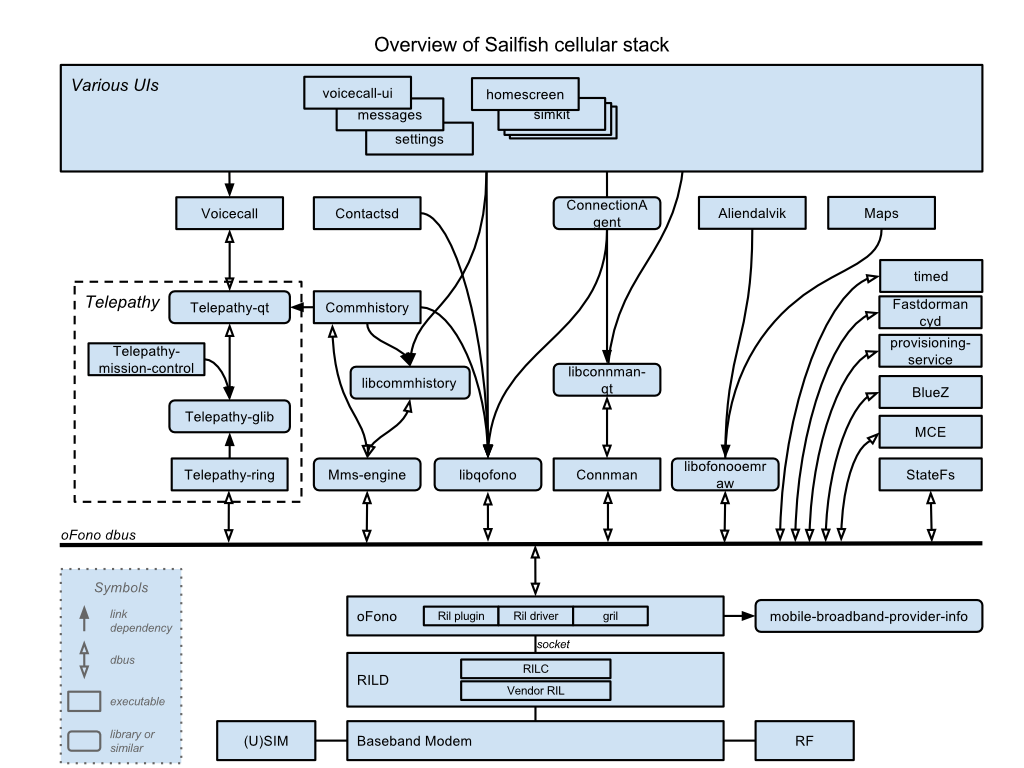
\includegraphics[width=0.5\textwidth]{Images/cellulardiagram}
  \caption{Diagram structuur telefonie SailfishOS. Bron: \styledhref{https://docs.sailfishos.org/Reference/Core_Areas_and_APIs/Networking/Cellular_Telephony_Architecture/}{docs.sailfish.org}}
  \label{fig:cellulardiagram}
  \end{figure}
  

% Sprint 5 waydroid taken
\begin{tcolorbox}[colback=white, coltitle=black, colframe=\userstorycolor, title=\textbf{User Story: }Als developer wil ik Waydroid als package kunnen bouwen\, zodat er android apps op de telefoon gerund kunnen worden.]
\begin{table}[H]
    \centering
  \begin{tabularx}{1\textwidth}{|X|X|}
    \hline
    \cellcolor[HTML]{ffcc99} \textbf{Taak} & \cellcolor[HTML]{ffcc99} \textbf{Acceptatie Criteria} \\ 
    \hline
    Onderzoeken naar mogelijkheden om Waydroid op de telefoon te krijgen & 
      \begin{enumerate}[leftmargin=.4cm, topsep=0cm, itemsep=.2cm]
        \item Er is een concrete manier gevonden om Waydroid te kunnen installeren op de Fairphone
      \end{enumerate}
    \\
    \hline
    Waydroid installeren op telefoon met sailfishOS:Chum & 
      \begin{enumerate}[leftmargin=.4cm, topsep=0cm, itemsep=.2cm]
        \item De Waydroid applicatie is geïnstalleerd op de Fairphone.
      \end{enumerate}
    \\
    \hline
    Onderzoek doen naar binder nodes & 
      \begin{enumerate}[leftmargin=.4cm, topsep=0cm, itemsep=.2cm]
        \item Er is duidelijk wat een binder node is en hoe deze samenwerken met Waydroid. 
        \item Er is een kort document dat een basisbegrip over binder nodes geeft voor de rest van het team.
      \end{enumerate}
    \\
    \hline
    
  \end{tabularx}
  \caption{User Story: Waydroid}
\label{table:it5:story_waydroid}
\end{table}
\end{tcolorbox}


\section{User Stories \& Taken}
\begin{tcolorbox}[colback=white, coltitle=black, colframe=\learningstorycolor, title=\textbf{Learning Story: }Als ontwikkelaar wil ik weten wat de rol van connman is in 4G\, zodat ik kan uitzoeken of het mobiele data probleem ligt bij connman.]
  \par\smallskip 
  Tijdens het onderzoeken van connman en de errors die zich opdeden, stuitte ik op error 4100 in de ofono logs.
  Toen ik dit onderzocht, kon ik niks vinden dat voor ons van toepassing was.
  Ik besprak dit met mijn groepsgenoot, Remy, en hij zei dat hij wel een post had gevonden op github met dezelfde error.
  Hierin werd gezegd dat dummy\_net installeren het zou kunnen oplossen.

  \begin{table}[H]
      \centering
    \begin{tabularx}{1\textwidth}{|X|X|}
      \hline
      \cellcolor[HTML]{ffcc99} \textbf{Taak} & \cellcolor[HTML]{ffcc99} \textbf{Acceptatie Criteria} \\ 
      \hline
      Uitzoeken wat connman is & Er is een begrip over wat connman is. \\ 
      \hline 
      Connman configuraties doorspitten & 
      \begin{enumerate}[leftmargin=.4cm, topsep=0cm, itemsep=.2cm]
        \item De standaard configuraties zijn gelezen. 
        \item De configuraties gezet in SailfishOS zijn bekeken en vergeleken met de standaard configuraties.
        \item Verschillen zijn onderzocht.
      \end{enumerate} \\ 
      \hline
      Connman logs onderzoeken & 
      \begin{enumerate}[leftmargin=.4cm, topsep=0cm, itemsep=.2cm]
        \item Er is gezocht naar errors in de connman logs.
        \item Potentiële errors zijn genoteerd. 
      \end{enumerate}\\
      \hline
      Proberen te verbinden met mobiele data met connmanctl & 
      Er is gekeken of er alsnog handmatig verbinding gemaakt kan worden met connmanctl. \\ 
      \hline
      Uitzoeken waarom we geen IP adres krijgen & 
      \begin{enumerate}[leftmargin=.4cm, topsep=0cm, itemsep=.2cm]
        \item Er is gezocht naar wat er nodig is om een IP adres te krijgen in mobiele data.
        \item Er zijn concrete punten gevonden om verder te onderzoeken.
      \end{enumerate} \\

      \hline
      Ofono log viewer gebruiken om error connman verder uit te zoeken & 
      \begin{enumerate}[leftmargin=.4cm, topsep=0cm, itemsep=.2cm]
        \item Ofono log viewer app is geinstalleerd.
        \item Connmanctl connect is gebruikt om geprobeerd te verbinden.
        \item Eventuele errors zijn genoteerd.
      \end{enumerate} \\
      \hline
      Ofono error 4100 onderzoeken & De ofono error 4100 is onderzocht en er zijn potentiële oplossingen gevonden. \\
      \hline
    \end{tabularx}
    \caption{Learning Story: Connman}
  \label{table:it4:story_connman}
  \end{table}
  \end{tcolorbox}

\begin{tcolorbox}[colback=white, coltitle=black, colframe=\userstorycolor, title=\textbf{User Story: }Als gebruiker wil ik graag met de Fairphone mobiele data kunnen gebruiken\, zodat ik ook onderweg internet kan gebruiken.]
  \par\smallskip 
    Ik probeerde dummy\_netd te installeren op de telefoon. Dit werkte. We wilden graag dat dit automatisch al in de OS zat, zodat 4G gewoon werkte zonder aanpassingen te maken.
    Dus downloadde ik dummy\_netd in de build environment. Dit werkte niet. 
    Daan wees mij op een hoofdstuk in de HADK porter's guide waar werd gepraat over patterns.
    Hierin stond dat je middleware packages aan de patterns moest toevoegen, zodat het werd meegebouwd.
    Dit heb ik gedaan en, na het bouwen van de images, werkte 4G perfect.

  \begin{table}[H]
      \centering
    \begin{tabularx}{1\textwidth}{|X|X|}
      \hline
      \cellcolor[HTML]{ffcc99} \textbf{Taak} & \cellcolor[HTML]{ffcc99} \textbf{Acceptatie Criteria} \\ 
      \hline
      Dummy\_netd installeren op de telefoon & De dummy\_netd package is geïnstalleerd op de telefoon. \\
      \hline 
      Testen of de dummy\_netd package installeren de error oplost & Er is geconstateerd of de dummy\_netd package installeren de errors oplost. \\
      \hline 
      Onderzoeken hoe we de package kunnen meebouwen via de build environment & Er is onderzocht hoe we de package moeten meebouwen, zodat deze in de sailfishos image komt te staan. \\ 
      \hline 
      Dummy\_netd installeren in de build environment & 
      \begin{enumerate}[leftmargin=.4cm, topsep=0cm, itemsep=.2cm]
        \item Dummy\_netd is gedownload van de github mer\_hybris/dummy\_netd.
        \item De package is geïnstalleerd via zypper.
        \item Er is een nieuwe image gebouwd.
        \item Er is gecontroleerd of dummy\_netd is meegebouwd.
      \end{enumerate} \\
      \hline
      Dummy\_netd toevoegen aan pattern bestanden & 
      \begin{enumerate}[leftmargin=.4cm, topsep=0cm, itemsep=.2cm]
        \item Dummy\_netd is toegevoegd als dependency in de pattern bestanden.
        \item Er is een nieuwe image gebouwd.
        \item Er is gecontroleerd of dummy\_netd is meegebouwd.
      \end{enumerate} \\
      \hline
    \end{tabularx}
    \caption{User Story: Mobiele Data}
  \label{table:it4:story_mobiledata}
  \end{table}
  \end{tcolorbox}



\chapter{Sprint 5}
\section{Algemene Informatie}
\begin{table}[H]
\begin{tabularx}{0.6\textwidth}{|X|X|}
  \hline
  \cellcolor[HTML]{99ccff} \textbf{Periode:} & 2023-11-13 t/m 2023-11-24 \\ 
  \hline
  \cellcolor[HTML]{99ccff} \textbf{Aantal taken:} & 7 \\ 
  \hline
  \cellcolor[HTML]{99ccff} \textbf{Totaal uren:} & 48 \\ 
  \hline
\end{tabularx}
\caption{Informatie Tabel}
\label{table:it5:general}
\end{table}
In sprint 5 heb ik vooral gewerkt aan het installeren van Waydroid.
We stuitten veel op problemen met binder nodes. Tijdens sprint 5 heb ik veel research gedaan naar binder nodes.
Ook heb ik de werkende images van vorige sprint gereleased op verschillende fora, waar ook de releases van het vorige team staan.


\section{User Stories \& Taken}

% Sprint 5 waydroid taken
\begin{tcolorbox}[colback=white, coltitle=black, colframe=\userstorycolor, title=\textbf{User Story: }Als developer wil ik Waydroid als package kunnen bouwen\, zodat er android apps op de telefoon gerund kunnen worden.]
  \begin{table}[H]
      \centering
    \begin{tabularx}{1\textwidth}{|X|X|}
      \hline
      \cellcolor[HTML]{ffcc99} \textbf{Taak} & \cellcolor[HTML]{ffcc99} \textbf{Acceptatie Criteria} \\ 
      \hline
      Onderzoeken naar mogelijkheden om Waydroid op de telefoon te krijgen & 
        \begin{enumerate}[leftmargin=.4cm, topsep=0cm, itemsep=.2cm]
          \item Er is een concrete manier gevonden om Waydroid te kunnen installeren op de Fairphone.
        \end{enumerate}
      \\
      \hline
      Waydroid installeren op telefoon met sailfishOS:Chum & 
        \begin{enumerate}[leftmargin=.4cm, topsep=0cm, itemsep=.2cm]
          \item De Waydroid applicatie is geïnstalleerd op de Fairphone.
        \end{enumerate}
      \\
      \hline
      Onderzoek doen naar binder nodes & 
        \begin{enumerate}[leftmargin=.4cm, topsep=0cm, itemsep=.2cm]
          \item Er is duidelijk wat een binder node is en hoe deze samenwerken met Waydroid. 
          \item Er is een kort document dat een basisbegrip over binder nodes geeft voor de rest van het team. (Zie \ref{bijlage:bindernodes})
        \end{enumerate}
      \\
      \hline
      
    \end{tabularx}
    \caption{User Story: Waydroid}
  \label{table:it5:story_waydroid}
  \end{table}
  \end{tcolorbox}
  

\begin{tcolorbox}[colback=white, coltitle=black, colframe=\userstorycolor, title=\textbf{User Story: }Als opdrachtgever wil ik dat er altijd een actieve sailfishOS build beschikbaar is\, zodat gebruikers de laatste functionaliteiten kunnen gebruiken.]
\begin{table}[H]
    \centering
  \begin{tabularx}{1\textwidth}{|X|X|}
    \hline
    \cellcolor[HTML]{ffcc99} \textbf{Taak} & \cellcolor[HTML]{ffcc99} \textbf{Acceptatie Criteria} \\ 
    \hline
    Nieuwe release op GitHub aanmaken &
     \begin{enumerate}
      \item Er is een release aangemaakt op de GitHub repository met daarin de hybris boot image en de nieuwst werkende SailfishOS image.
     \end{enumerate}
      \\
    \hline 
    Nieuwe release post op XDA Forums maken & 
    \begin{enumerate}[leftmargin=.4cm, topsep=0cm, itemsep=.2cm]
      \item Er is een post gemaakt op de XDA Forums met daarin informatie over de nieuwste release.
      \item De post heeft een soortgelijke opmaak en structuur als \styledhref{https://xdaforums.com/t/lineageos-19-1-android-12l-signature-spoofing-ota-updates-for-s8-s8-note8.4370375/}{de LineageOS 19.1 Release}.
      \item De post is goedgekeurd door de opdrachtgever.
     \end{enumerate}
    \\ 
    \hline 
    Nieuwe release post op SailfishOS Forums maken & 
    \begin{enumerate}[leftmargin=.4cm, topsep=0cm, itemsep=.2cm]
      \item Er is een post gemaakt op de SailfishOS Forums met daarin informatie over de nieuwste release.
      \item De post heeft een soortgelijke opmaak en structuur als \styledhref{https://xdaforums.com/t/lineageos-19-1-android-12l-signature-spoofing-ota-updates-for-s8-s8-note8.4370375/}{de LineageOS 19.1 Release}.
      \item De post is goedgekeurd door de opdrachtgever.
     \end{enumerate}
    \\ 
    \hline 
    Nieuwe release post op Fairphone Forums maken & 
    \begin{enumerate}[leftmargin=.4cm, topsep=0cm, itemsep=.2cm]
      \item Er is een post gemaakt op de Fairphone Forums met daarin informatie over de nieuwste release.
      \item De post heeft een soortgelijke opmaak en structuur als \styledhref{https://xdaforums.com/t/lineageos-19-1-android-12l-signature-spoofing-ota-updates-for-s8-s8-note8.4370375/}{de LineageOS 19.1 Release}.
      \item De post is goedgekeurd door de opdrachtgever.
     \end{enumerate}
    \\ 
    \hline 
        
  \end{tabularx}
  \caption{User Story: Nieuwe releases}
\label{table:it5:new_releases}
\end{table}
\end{tcolorbox}



\chapter{Sprint 6}
\section{Algemene Informatie}
\begin{table}[H]
\begin{tabularx}{0.6\textwidth}{|X|X|}
  \hline
  \cellcolor[HTML]{99ccff} \textbf{Periode:} & 2023-11-27 t/m 2023-12-08 \\ 
  \hline
  \cellcolor[HTML]{99ccff} \textbf{Aantal taken:} & 5 \\ 
  \hline
  \cellcolor[HTML]{99ccff} \textbf{Totaal uren:} & 48 \\ 
  \hline
\end{tabularx}
\caption{Informatie Tabel}
\label{table:it6:general}
\end{table}
Sprint 6 was een vrij langzame sprint. We liepen constant tegen problemen aan met Waydroid, specifiek over de binder nodes.
In de afgelopen sprint hebben we uitgezocht wat er gedaan moet worden om binder nodes werkend moeten krijgen, maar hiervan werkte uiteindelijk niks. 
We bleven tegen dezelfde error aanlopen.
Uiteindelijk hebben we een post gemaakt op de SailfishOS forums, waar we hulp vroegen aan de community. 
Voor het einde van de sprint hadden we helaas nog geen reacties hier op.
Ook hebben we hulp gevraagd aan onze opdrachtgever, die hier helaas ook geen verdere ideeën over had.
Daarnaast heb ik in deze sprint mijn teamgenoten nog geholpen bij wat errors die zich opdeden in Docker, maar hier hadden we geen aparte taak voor op het scrumboard.

\section{User Stories \& Taken}
% Sprint 6 
\begin{tcolorbox}[colback=white, coltitle=black, colframe=\userstorycolor, title=\textbf{User Story: }Als developer wil ik Waydroid als package kunnen bouwen\, zodat er android apps op de telefoon gerund kunnen worden.]
  \begin{table}[H]
      \centering
    \begin{tabularx}{1\textwidth}{|X|X|}
      \hline
      \cellcolor[HTML]{ffcc99} \textbf{Taak} & \cellcolor[HTML]{ffcc99} \textbf{Acceptatie Criteria} \\ 
      \hline 
      Nieuwe kernel met binder nodes bouwen & Er is een nieuwe kernel gebouwd met daarin de binder nodes geconfigureerd. \\
      \hline
      Nieuwe kernel met binder nodes testen &  
      \begin{enumerate}[leftmargin=.4cm, topsep=0cm, itemsep=.2cm]
        \item De gebouwde kernel is geflashed op de telefoon.
        \item Er is geconstateerd of Waydroid de binder nodes ziet en kan gebruiken.
      \end{enumerate}\\ 
      \hline 
      Vraag posten over probleem met binder nodes op Sailfish forums & \href{https://forum.sailfishos.org/t/the-fairphone-4-thread/17543/2?u=dimac4455}{Er is een post gemaakt} met de vraag over het binder node probleem. \\
      \hline 
      Vragen om hulp bij opdrachtgever & Er is gevraagd om ideeën voor verdere stappen aan de opdrachtgever. \\
      \hline       
    \end{tabularx}
    \caption{User Story: Waydroid}
  \label{table:it6:story_waydroid}
  \end{table}
  \end{tcolorbox}
  
\begin{tcolorbox}[colback=white, coltitle=black, colframe=\learningstorycolor, title=\textbf{Learning Story: }Als developer wil ik weten wat puddlejumper en vndjumper is\, zodat ik kan begrijpen hoe ik de binder nodes moet configureren.]
  \begin{table}[H]
      \centering
    \begin{tabularx}{1\textwidth}{|X|X|}
      \hline
      \cellcolor[HTML]{ffcc99} \textbf{Taak} & \cellcolor[HTML]{ffcc99} \textbf{Acceptatie Criteria} \\ 
      \hline 
      Googlen naar puddlejumper en vndjumper & Er is online gezocht naar referenties naar puddlejumper en vndjumper. \\
      \hline
    \end{tabularx}
    \caption{Learning Story: Puddlejumper}
  \label{table:it6:story_puddlejumper}
  \end{table}
  \end{tcolorbox}
  


\chapter{Bijlagen}
\section{Bijlage A - Binder Nodes}
\label{bijlage:bindernodes}
\begin{minipage}{\textwidth}
  \centering
  \fbox{
  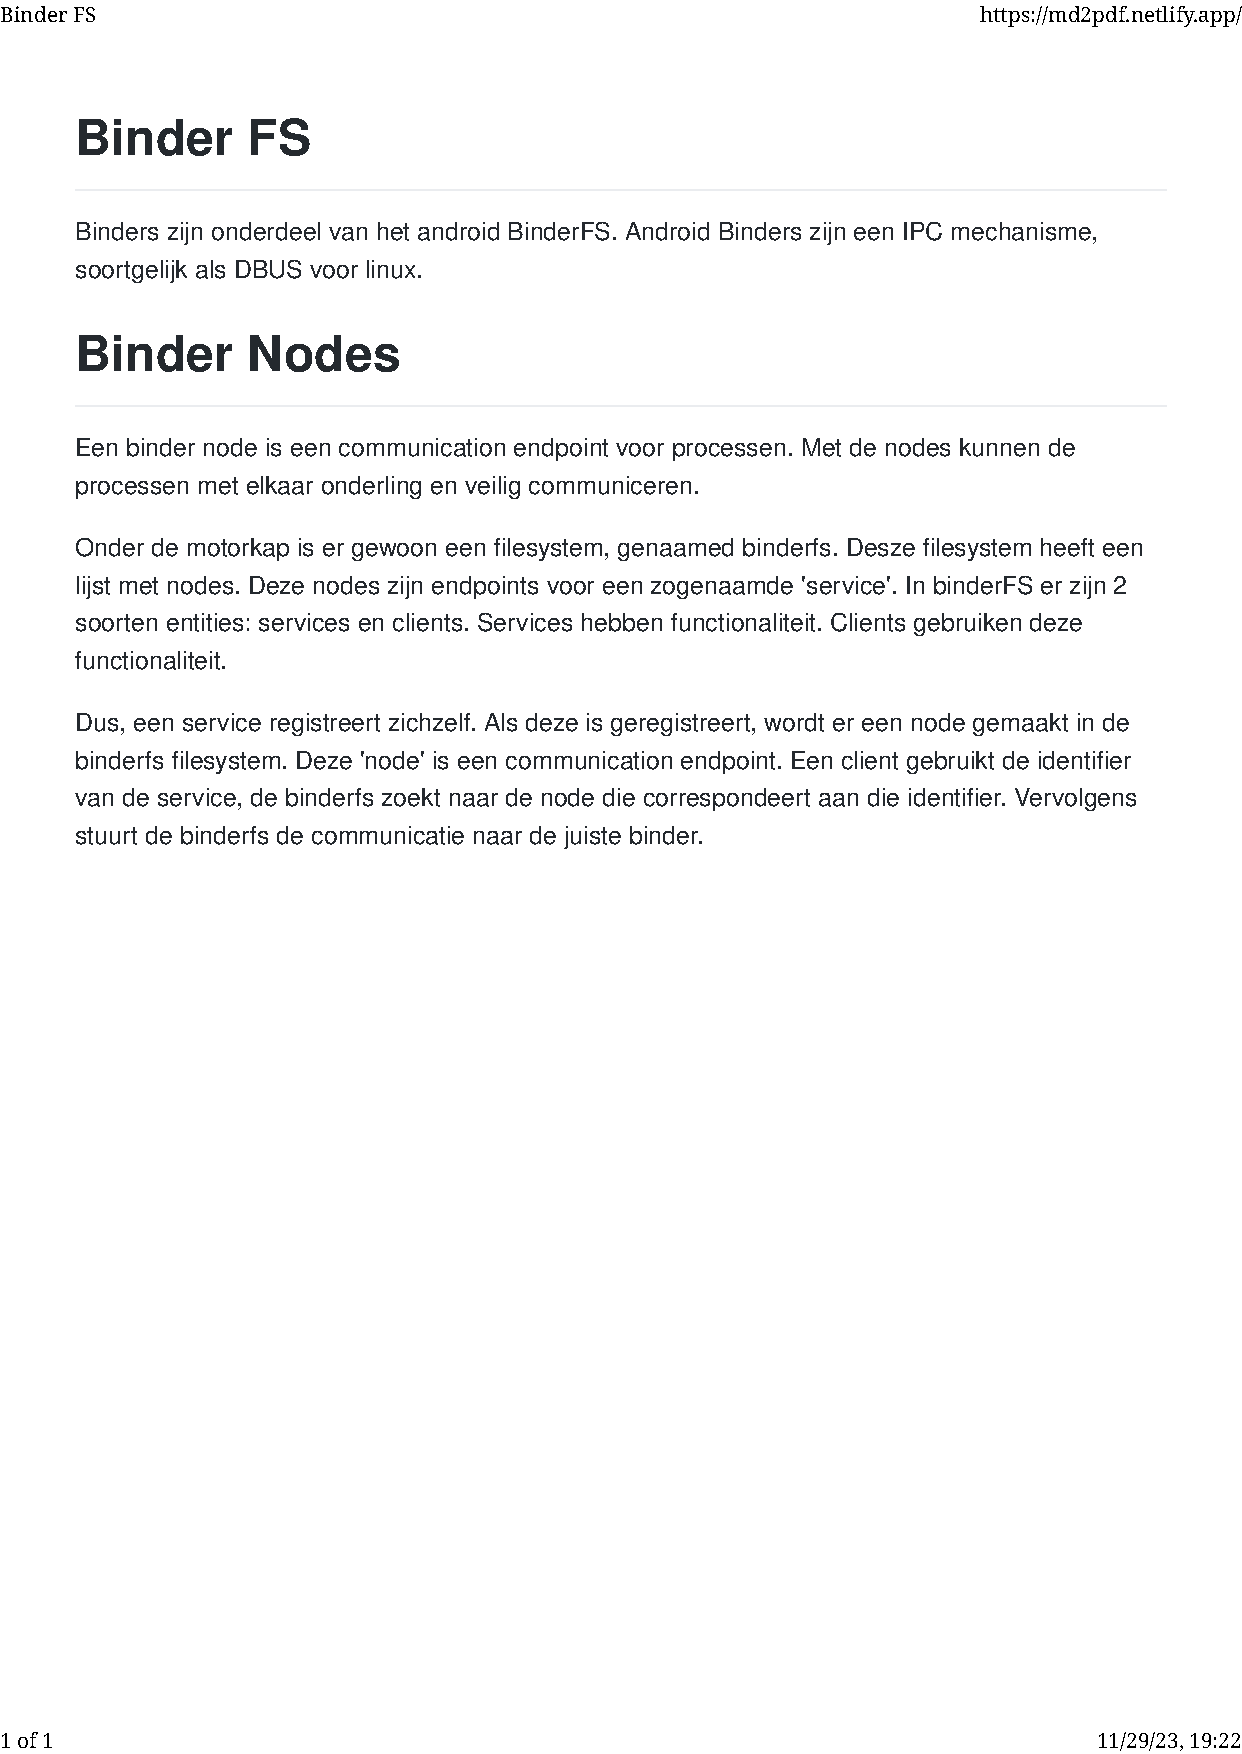
\includegraphics[page=1,scale=0.7]{Appendices/Binderfs.pdf}}
\end{minipage}
\clearpage
\section{Bijlage B - User Guide}
\label{bijlage:userguide}
\begin{minipage}{\textwidth}
  \centering
  \fbox{
  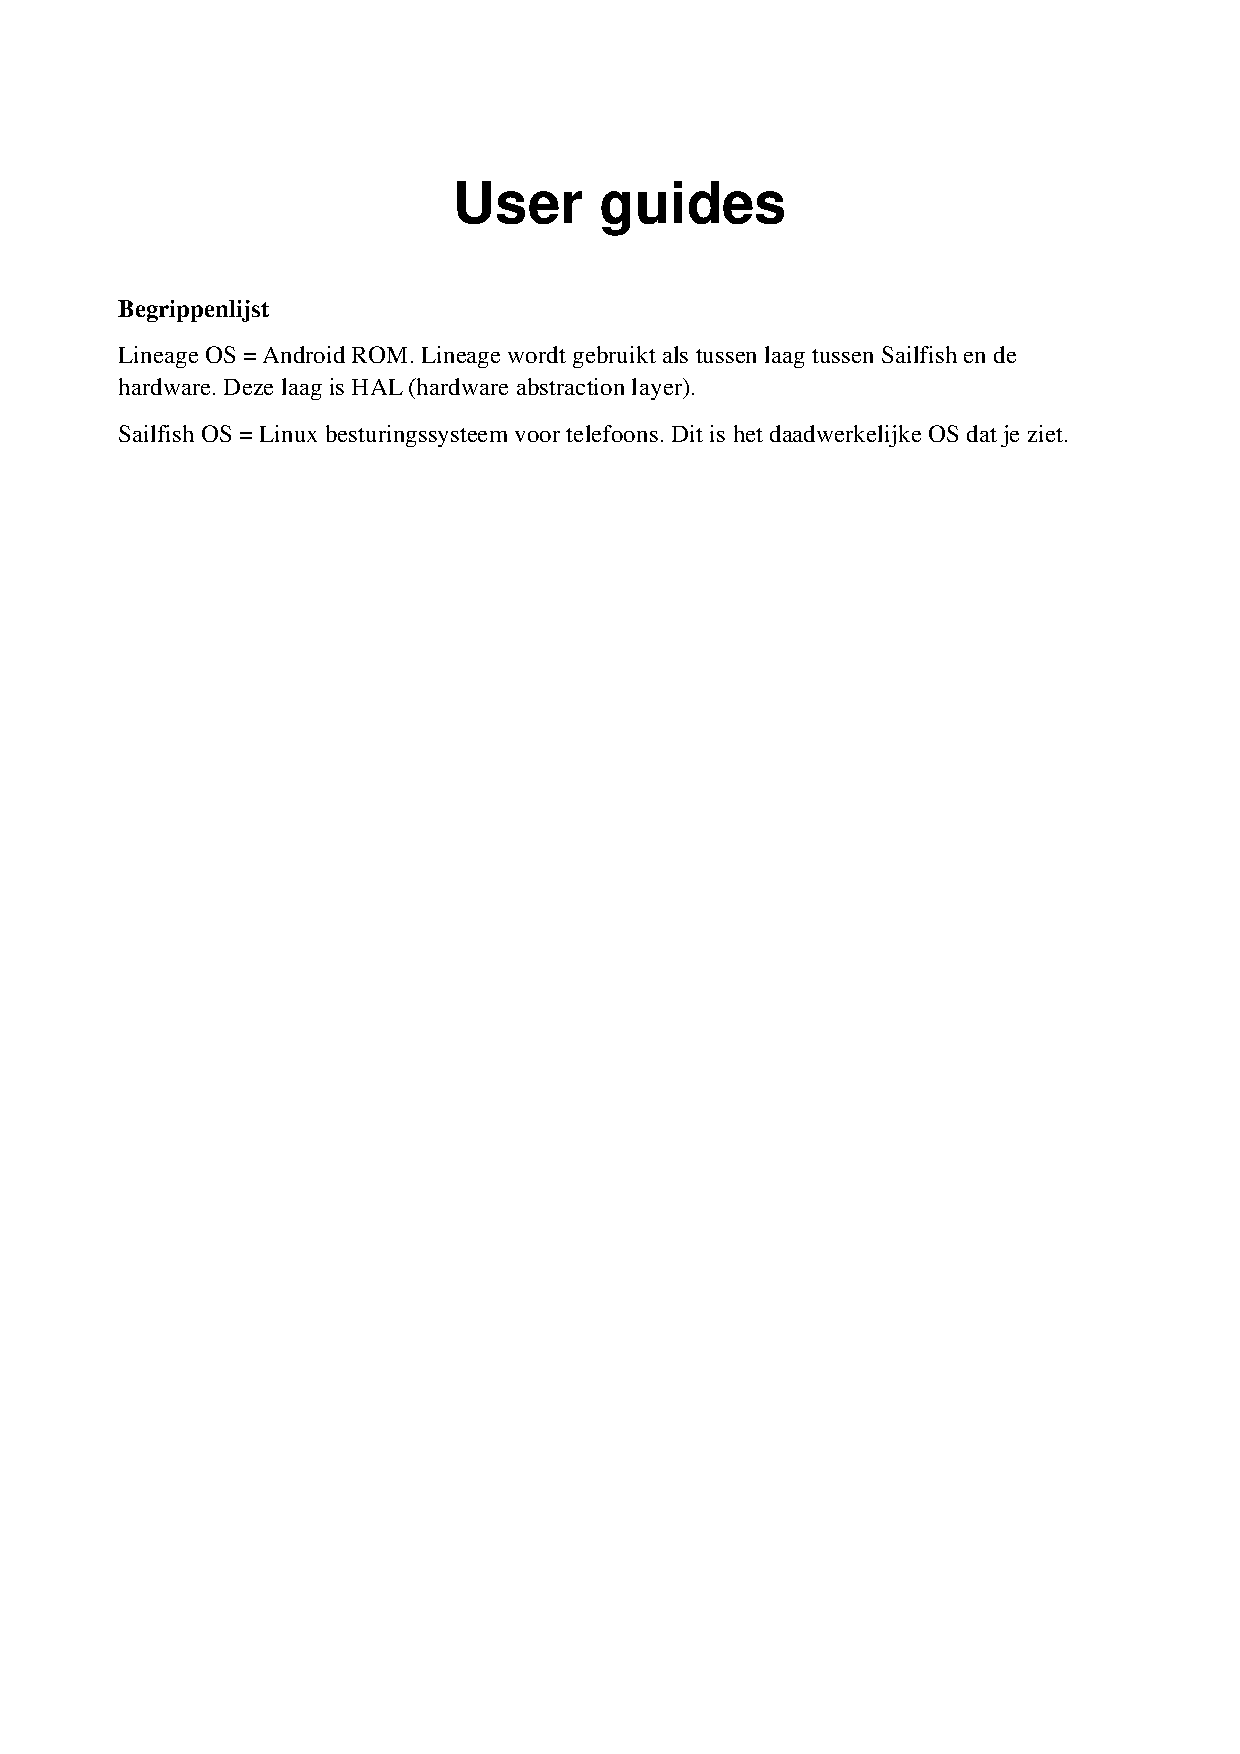
\includegraphics[page=1,scale=0.7]{Appendices/userguide.pdf}}
\end{minipage}
\includepdf[pages={2-5},scale=0.7,frame,pagecommand={}]{Appendices/userguide.pdf}


\end{document}